%!TEX TS-program = pdflatex
%!TEX root = tesi.tex
%!TEX encoding = UTF-8 Unicode

\chapter{Risultati Ottenuti}
\todo[inline]{sommario capitolo}
% descrizione architettura migliore e a chi ci siamo ispirati N.R.
\todo[inline]
{
  Preambolo sulla accuratezza dei modelli creati
  Problema dell'AE perché non fornisce accuratezza, come parametro di valutazione si è utilizzata la loss
  La loss non poteva essere usata come discrtiminatoe perché troppo poco sensibile all'errore di presenza-nonpreseena della colla
  Un altro criterio di valutazione era una verifica a mano della qualità della differenza conforme in out

  Descrivere architettura migliore
  Descrivere post-processing a valle
}

\clearpage
\section{Il nostro obbiettivo TODO}
In figura~\ref{fig:obbiettivo_in_out_diff} sono riportate tre immagini per chiarire in che modo gli \textit{autoencoder} sono stati sfruttati per classificare Conformi e Scarti.
La figura~\ref{fig:obbiettivo_in} illustra uno Scarto.
L'immagine riportata in figura~\ref{fig:obbiettivo_out} è quella che si vorrebbe ottenere dall'AE a partire dallo Scarto appena illustrato.
Notare come si vorrebbe che il pezzo fosse riprodotto il più fedelmente possibile, ma che l'informazione della colla venisse rimossa.
In questo modo sarebbe possibile effettuare una differenza \textit{pixel} per \textit{pixel} tra immagine in ingresso ed immagine in uscita (detta anche ricostruita) ottenendo così un risultato simile a quello in figura~\ref{fig:obbiettivo_diff}.

Nel caso migliore possibile la classificazione verrebbe effettuata verificando se nell'immagine differenza tutti i valori sono zero.
Ossia l'immagine in ingresso appartiene alla classe Conforme ed è stata ricostruito alla perfezione.
Dato che ci si aspetta che l'\textit{autoencoder} non ricostruisca la colla nell'immagine in uscita, nell'immagine differenza ci sarà un'area di \textit{pixel} con valori in assoluto maggiori di zero.

È impossibile che l'\textit{autoencoder} raggiunga una precisione così alta, infatti è molto più infatti che l'immagine ricostruita sia soltanto un'approssimazione dell'immagine in ingresso.
Si ricorda che molto probabilmente l'AE rimuoverà tutte quelle caratteristiche particolari di un pezzo (graffi, macchie, \dots ), perché sono rumore rispetto ad una carcassa media.

Quindi si può affermare che la classificazione è divisa in due parti: nella prima l'immagine viene elaborata dall'\textit{autoencoder}; nella seconda l'immagine in ingresso e quella in uscita vengono confrontate, questa parte prende il nome di \textit{post-processing}.
L'effettiva classificazione viene eseguita in quest'ultima parte.

\begin{figure}[ht] % TODO
  \begin{center}
    \begin{tabular}{ccc}

      \begin{subfigure}{.3\linewidth}
        \centering\includegraphics[width=\textwidth]{example-image}
        \caption{Immagine in ingresso}
        \label{fig:obbiettivo_in}
      \end{subfigure} &

      \begin{subfigure}{.3\linewidth}
        \centering\includegraphics[width=\textwidth]{example-image}
        \caption{Immagine ricostruita}
        \label{fig:obbiettivo_out}
      \end{subfigure} &

      \begin{subfigure}{.3\linewidth}
        \centering\includegraphics[width=\textwidth]{example-image}
        \caption{Immagine differenza}
        \label{fig:obbiettivo_diff}
      \end{subfigure}

    \end{tabular}
    \caption{TODO in out diff}
    \label{fig:obbiettivo_in_out_diff}
  \end{center}
\end{figure}

\clearpage
\section{Metriche di valutazione}
Definire delle metriche per stabilire quali architetture preformassero meglio è stata una parte critica.
Infatti gli \textit{autoencoder} potevano essere confrontati solo tramite due criteri: uno numerico, ossia la \textit{MSE Loss} ottenuta durante l'allenamento, ed uno qualitativo, cioè osservare la qualità generale delle immagini generate.
Purtroppo nessuna delle due metriche permette di ottenere delle percentuali esatte sull'accuratezza delle classificazioni.
Tali dati numerici sono stati ottenuti soltanto quando le immagini differenza sono risultate soddisfacenti e si è quindi potuto sviluppare l'algoritmo di \textit{post-processing}.
\todo[inline]{c'è da dire altro?}


\clearpage
\section{Architettura del modello}
\todo[inline]{dire meglio}
Dopo molte iterazioni e tentativi si è ottenuta l'architettura in figura~\ref{fig:ae16_arch}\footnote{L'immagine è stata generata usando \url{https://github.com/HarisIqbal88/PlotNeuralNet}}.
Elenchiamo le sue caratteristiche principali:
\begin{itemize}
  \item l'immagine in ingresso è in scala di grigi e di lato $200$ \textit{pixel};

  \item ogni strato convolutivo o convolutivo trasposto ha filtri di dimensione $5$x$5$, ha \textit{stride} pari a $1$, non ha nessun \textit{padding} e tutti (tranne il primo e l'ultimo strato) hanno $ch_{in}=ch_{out}=32$.
    %Il primo strato ha un canale ingresso, dato che l'\textit{input} non è a colori,
    Inoltre tutti i \textit{layer} utilizzano la funzione di attivazione \textit{ReLU}, fatta eccezione per l'ultimo in cui è presente la funzione sigmoidea.
    Infatti le immagini, prima di essere passate alla rete, vengono normalizzate in $[0,1]$, cioè facilita i calcoli effettuati all'interno dell'\textit{autoencoder}.
    L'output della rete, appartenente a $[0,1]$, verrà mappato nuovamente nell'intervallo $[0,255]$.

  \item tutti i \textit{max-pool layer} hanno sia il filtro che il passo pari a 2;

  \item il primo strato denso prende un vettore di $24*24*32=18432$ valori e lo mappa in uno spazio $2000$-dimensionale.
    Questa corrisponde alla massima compressione dell'informazione;

  \item il secondo strato denso effettua l'operazione opposta, mappando il vettore dello spazio latente in uno che possa avere le dimensioni di $24*24*32$.

\end{itemize}
%TODO fare tabella con i parametri di ogni strato?
Complessivamente la rete deve imparare  $73 832 000$ parametri.
Di questi metà si trovano nell'\textit{encoder} e metà nel \textit{decoder}.
Questo valore potrebbe sembrare grande ma, osservando che la VGG11~\cite{vgg} ha più di 130 milioni di parametri, risulta ragionevole.
Si fa notare che la maggior parte dei parametri è contenuto nei due strati densi.
Sappiamo che il numero di parametri di uno strato è dato da $n * m$ con $n$ ed $m$le dimensioni dei vettori in ingresso ed in uscita.
Nel nostro caso abbiamo due strati da $18432 * 2000 = 36 864 000$ parametri l'uno.
I quattro \textit{layer} convolutivi e convolutivi trasposti da 32 canali in ingresso ed in uscita hanno $25600$ parametri ciascuno.
\todo[noline]{cos'altro da dire?}

\begin{figure}[ht]
  \begin{center}
    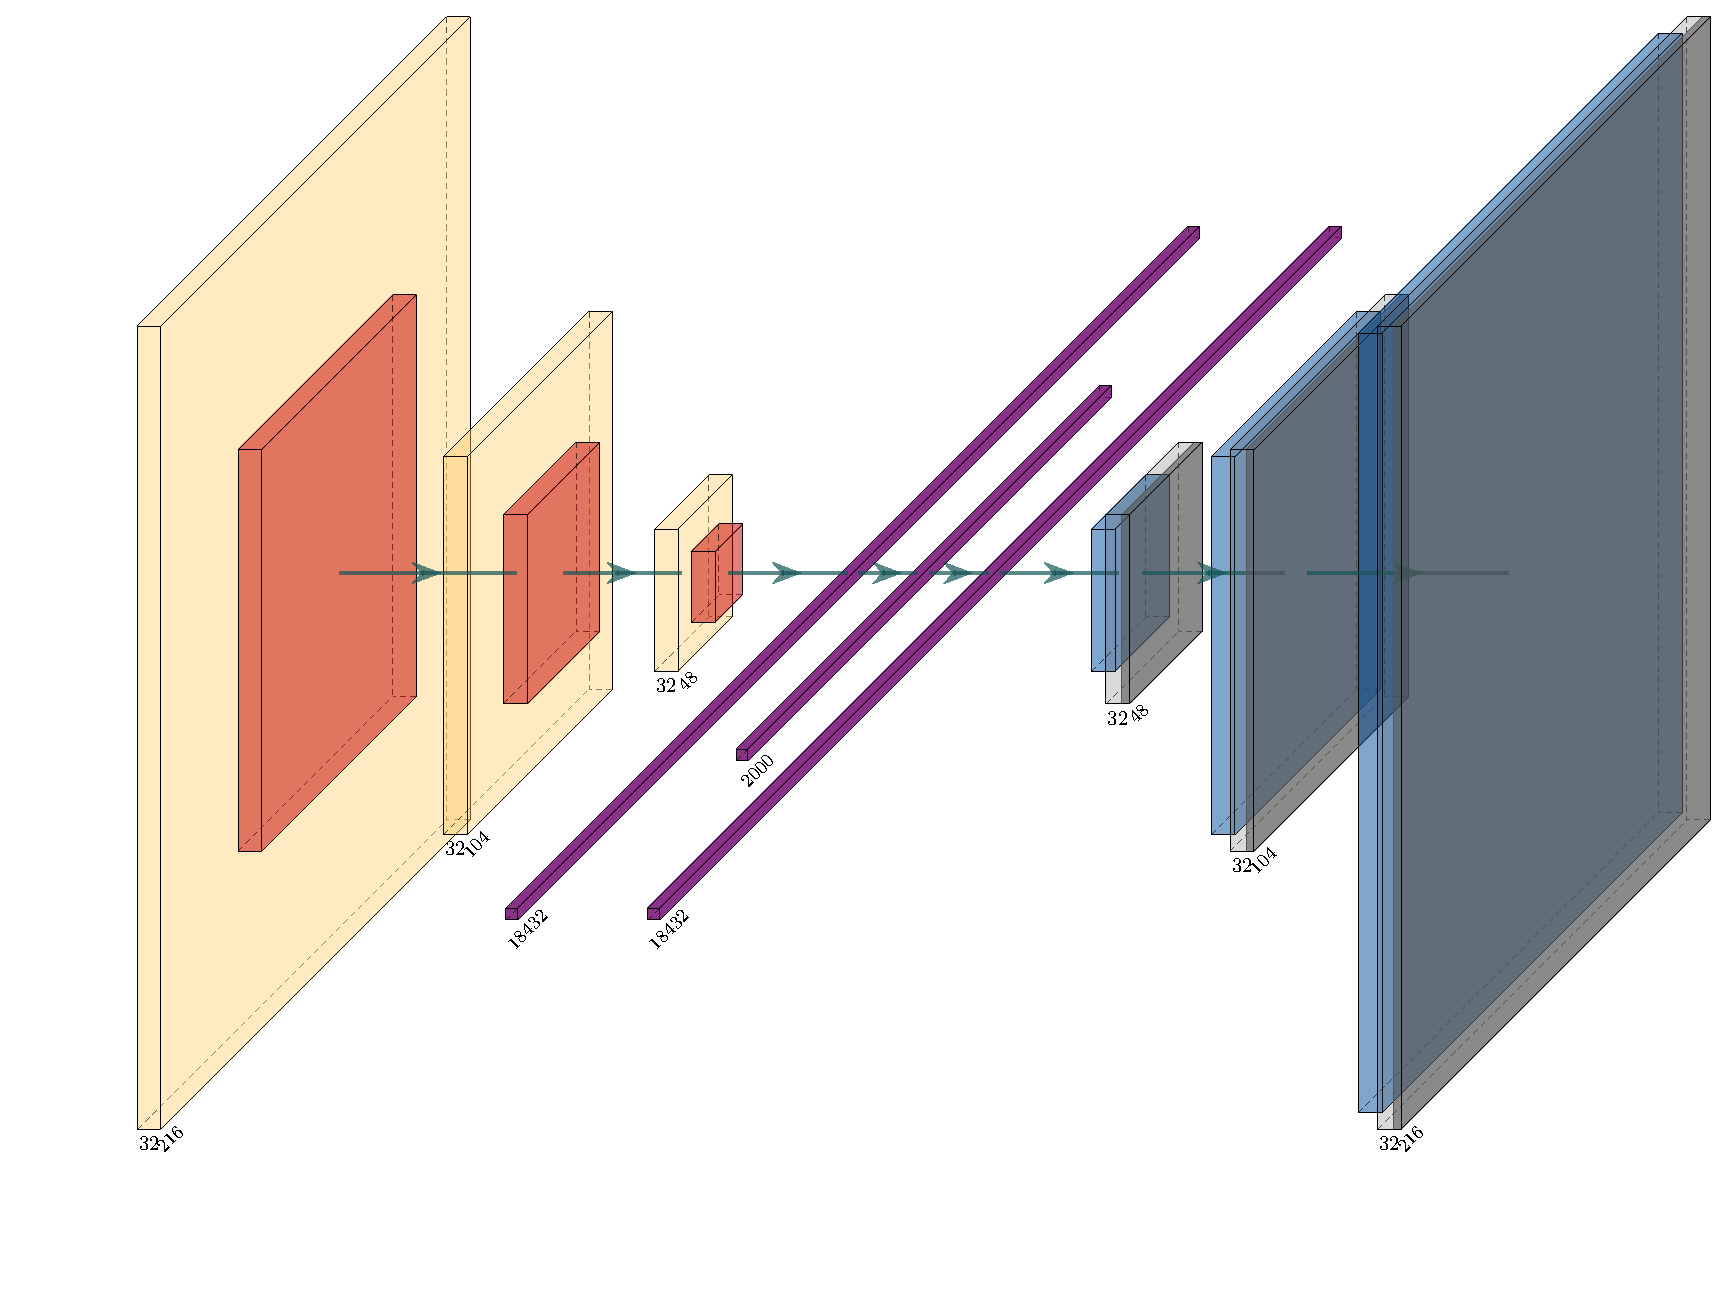
\includegraphics[width=\textwidth]{ae16}
    \caption{TODO architettura della rete}
    \label{fig:ae16_arch}
  \end{center}
\end{figure}
\todo[noline]{rifai disegno architettura i conv trans sono svaccati}

\clearpage

Durante l'allenamento si è utilizzata la \textit{MSE Loss} confrontando lo scarto tra l'immagine in ingresso e l'immagine ricostruita.
Nel grafico in figura~\ref{fig:loss_plot} si può notare come la loss scenda in modo repentino nelle prime 5 epoche per poi stabilizzarsi.
Il tasso di apprendimento\footnote{In inglese \textit{learning rate}}



\begin{figure}[ht]
  \begin{center}
    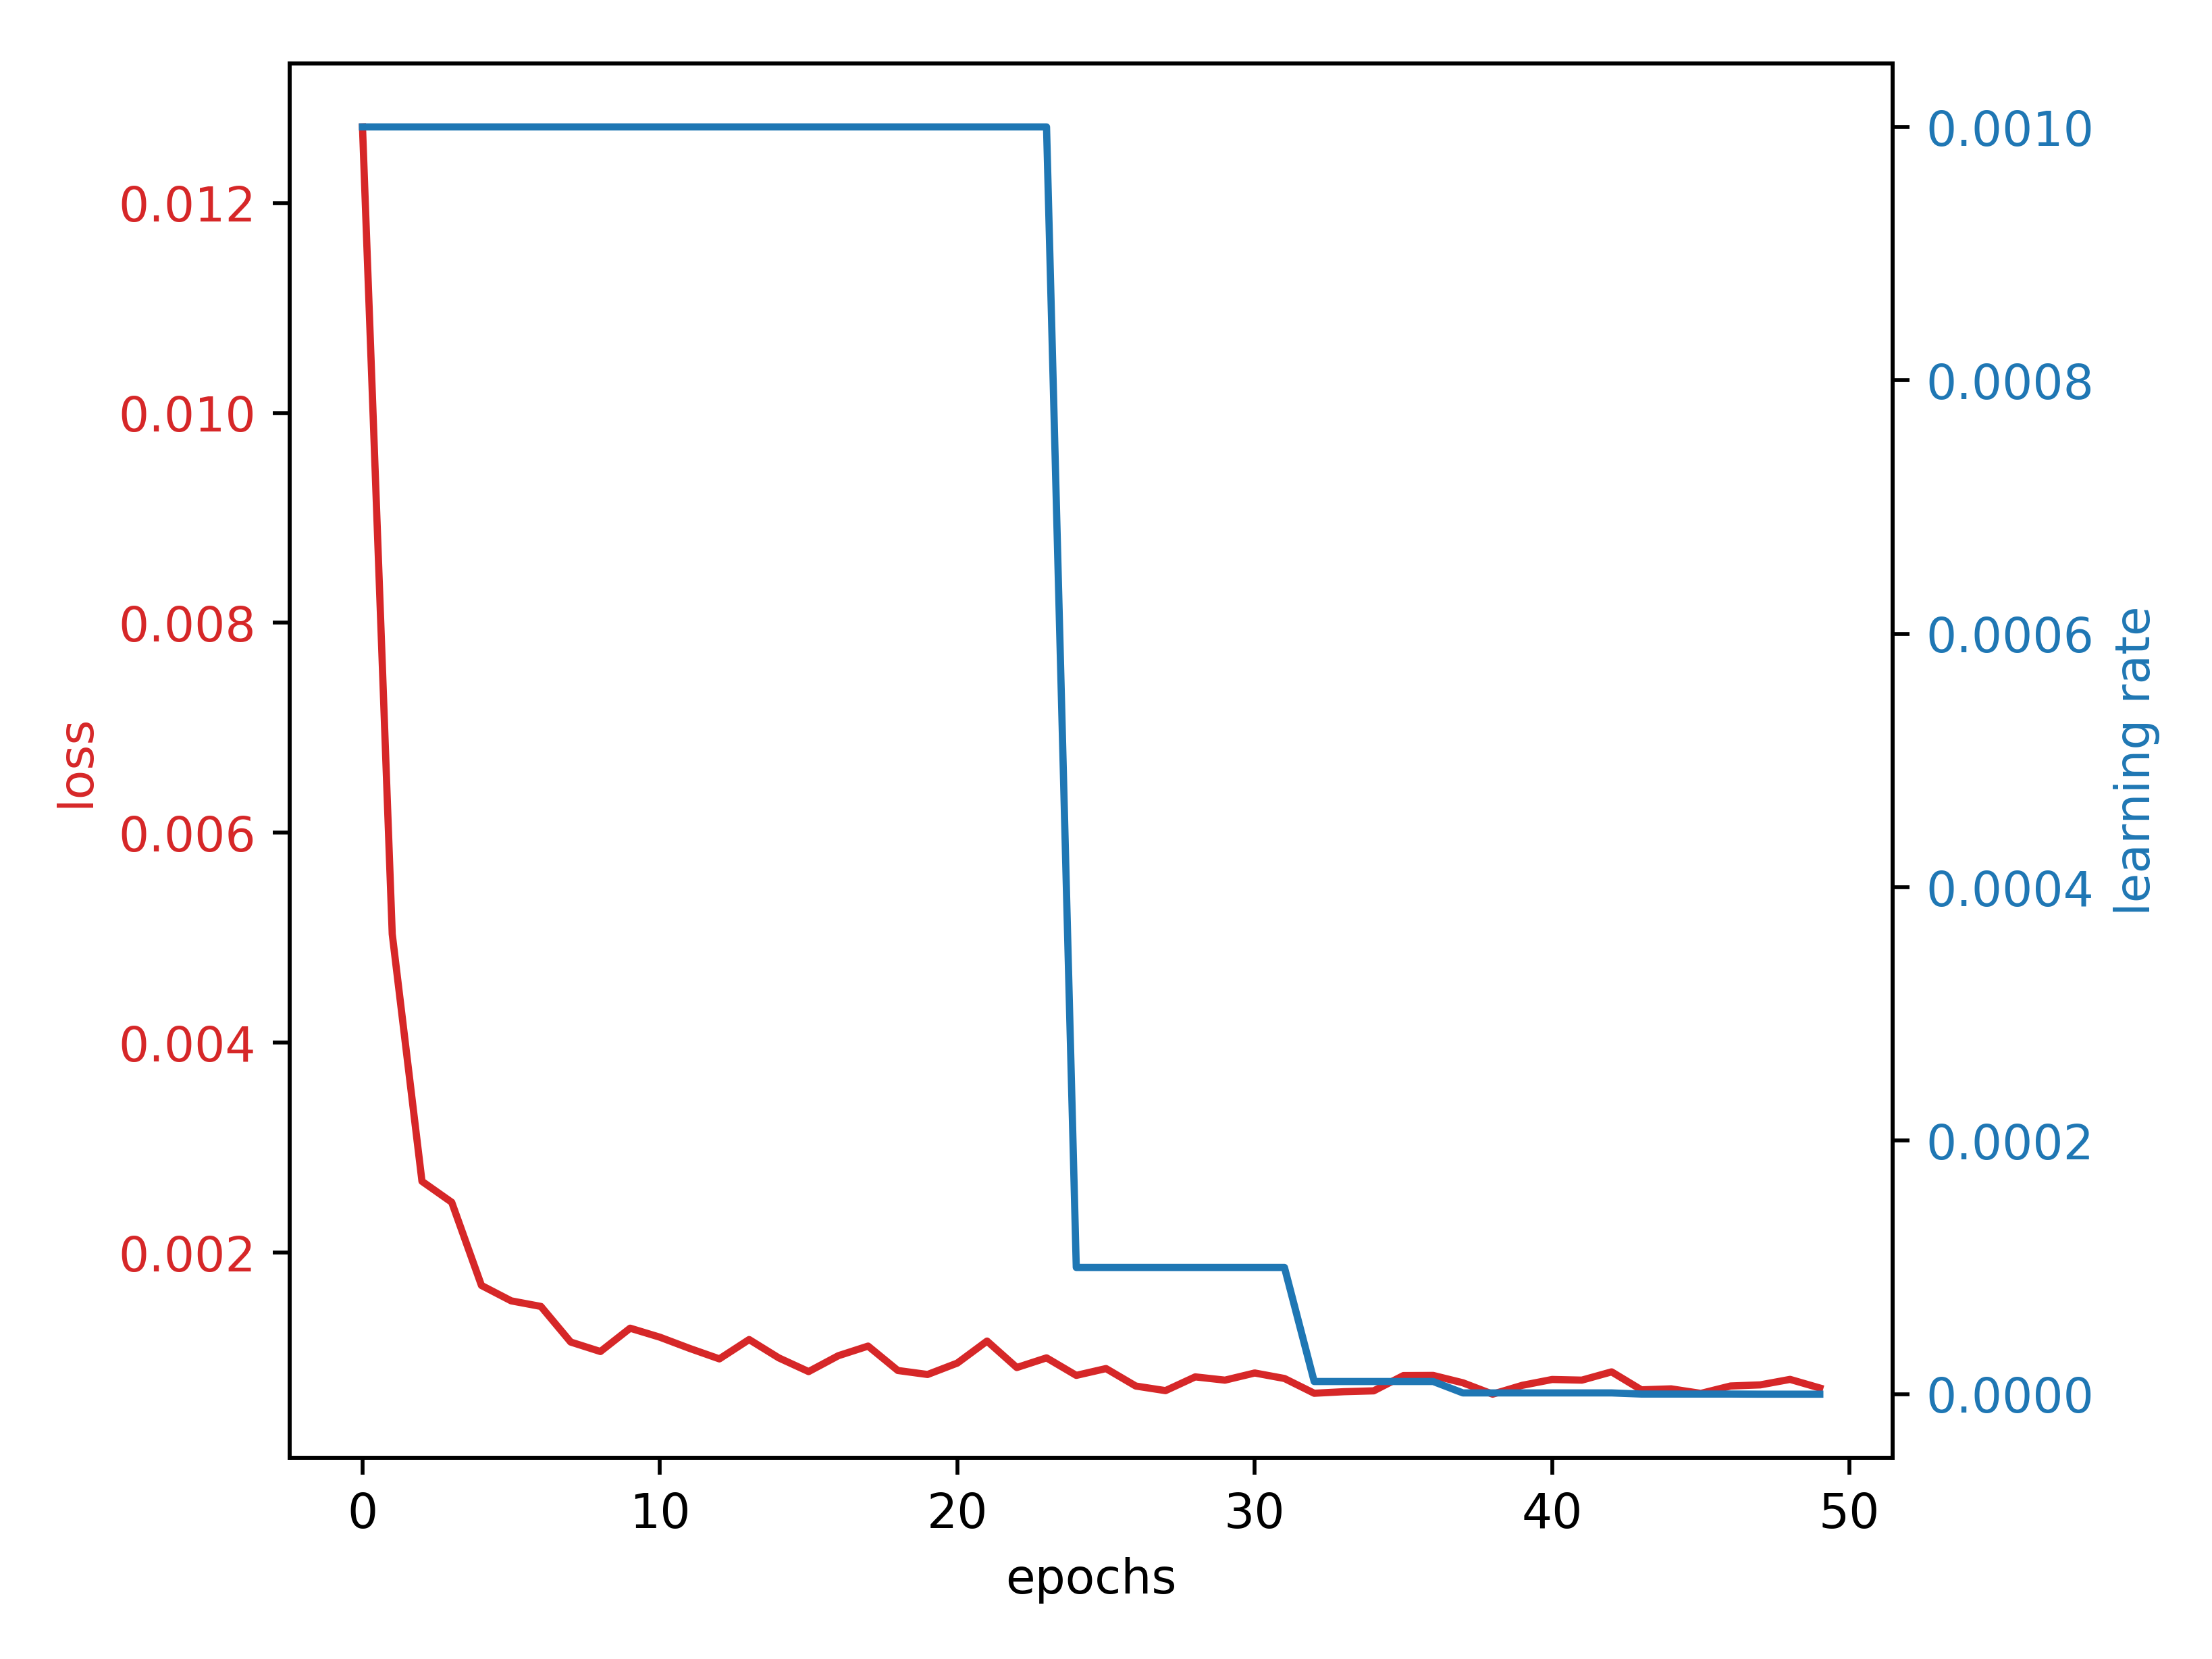
\includegraphics[width=0.8\textwidth]{loss_plot}
    \caption{TODO plot della loss}
    \label{fig:loss_plot}
  \end{center}
\end{figure}

\clearpage
\section{Post-Processing}
